\chapter{一阶段乳腺钼靶分类检测模型simFaster R-CNN}\label{chap:stage1}
\section{目的}
考虑到两阶段模型存在训练耗时长、空间占用大、参数量众多难以调节、训练测试反复进行耗时长等问题。通过对乳腺钼靶数据的了解和检测模型的深入理解,本文着手设计更加轻便的一阶段模型,使得模型可以在检测并分类出恶性病灶的同时,能够学习到恶性和正常病灶之间的细微区别。对于医学上的医疗影像问题,这种同时存在恶性及正常样本的问题很多,具体在产业化、标准化中,也需要模型能够更加轻便高效。

两阶段模型的思路清晰,第一阶段重点学习恶性病灶特征,使得postive能够及时被检测分类,人为标注出negative中疑似恶性病灶区域,将带有疑似恶性病灶的negative与positive融合后再次训练,第二阶段着重于学习恶性病灶和疑似病灶之间的微弱区别,这种分阶段式的训练方式符合一般逻辑。

通过对损失函数的观察,发现损失函数占比较高的是Fast R-CNN的损失,而RPN网络的损失并不太高,这说明RPN网络能够较为充分地学习到物体(在本文中指的是病灶)的特征。原始的Faster R-CNN的RPN着重考虑能否区分出物体,其对物体的ground-truth在RPN训练之前就已给出,而完全忽略了RPN会产生大量的高度疑似物体的负anchors,在乳腺钼靶问题中这个问题尤为突出。由于存在大量高度疑似恶性病灶的negative(如图\ref{fig:data_all}所示)在RPN网络中没有及时筛选出,使得Fast R-CNN的输入数据存在大量带有干扰性的负anchor数据,进而影响模型的进一步区分这种差异的能力。

为此,综合损失函数和数据本身的特点,在进行一阶段模型设计时候,需要重点考虑模型的能够识别不同类之间的能力。在此基础上本文引入全新损失函数,对原始的Faster R-CNN进行改进,提出simFaster R-CNN,使得模型能够同时学习恶性病灶特征以及恶性和高度恶性病灶之间的区别,从而加快模型训练与学习。

\section{模型图}
simFaster R-CNN的网络结构如图\ref{fig:stage1_model}所示。
\begin{figure}[!htbp]
    \centering
    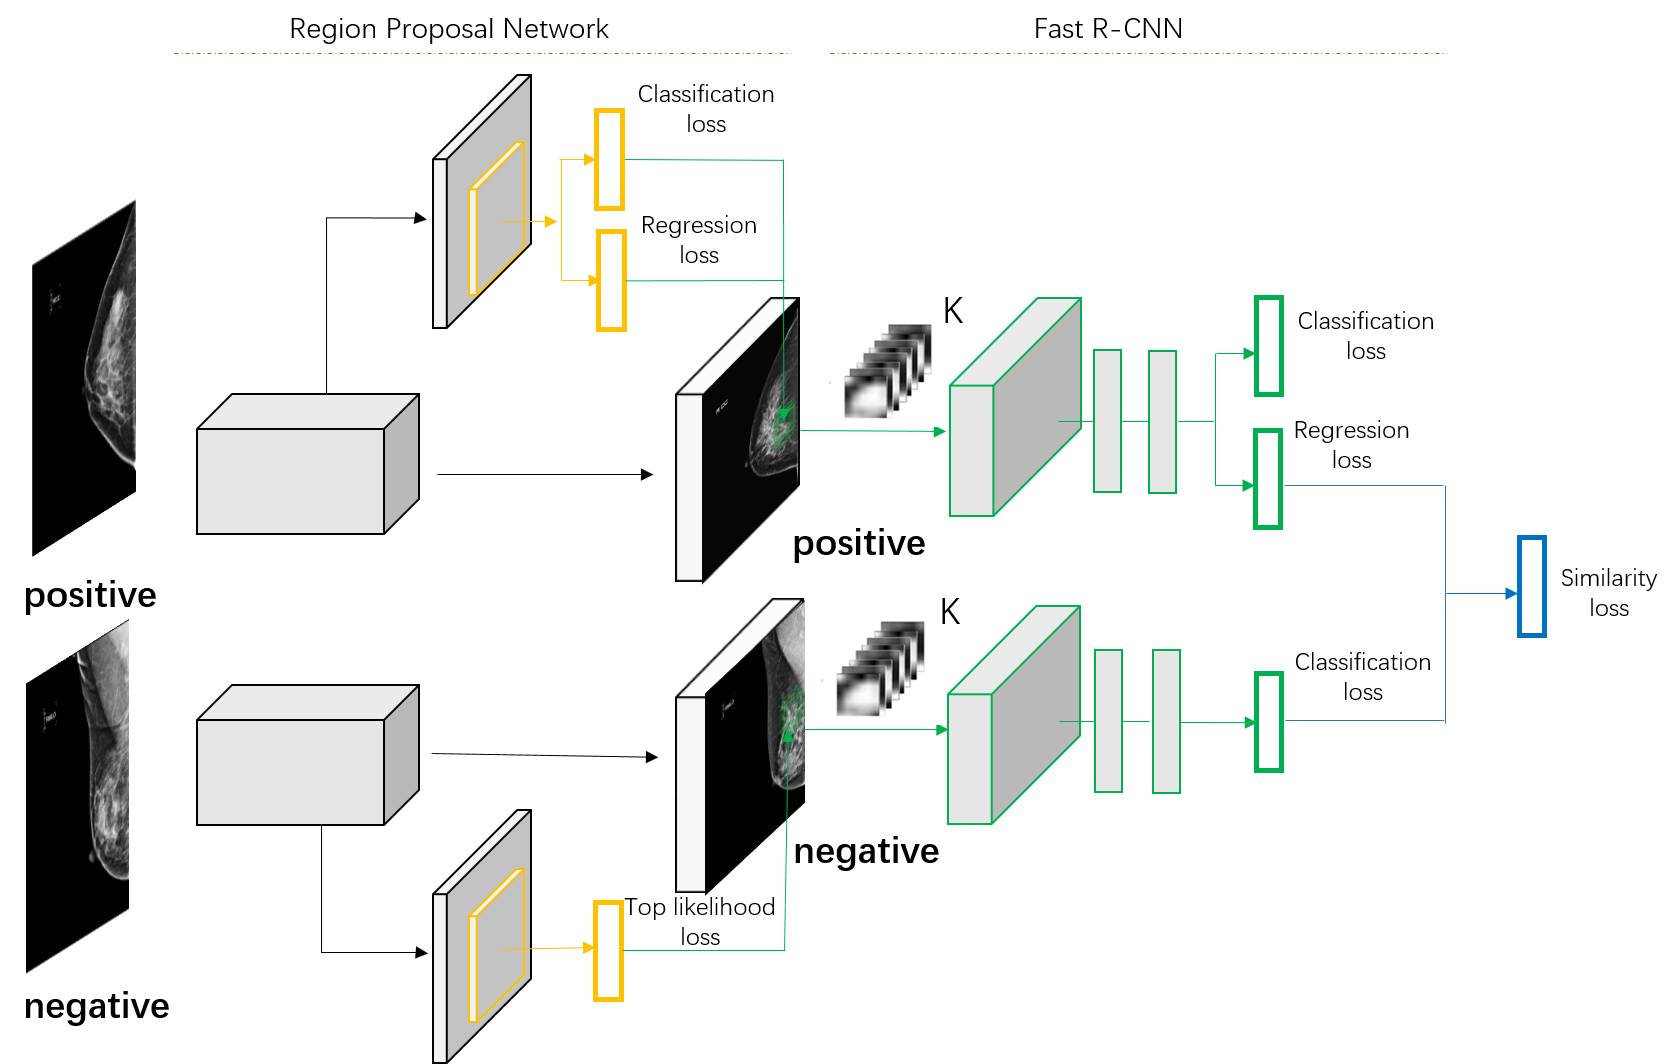
\includegraphics[width=1.0\textwidth]{stage1_model}
    \bicaption{simFaster R-CNN模型图}{Architecture of simFaster R-CNN}
    \label{fig:stage1_model}
\end{figure}

本模型是基于Faster R-CNN模型演变而来。主干部分不变,但输入变成相同数量的恶性和正常样本,二者经过共享的主干网络进行特征提取,获取到对应的特征,共享RPN网络。对恶性样本按照原始的Faster R-CNN的损失函数,对正常样本则是引入top likelihood loss。之后将二者生成的候选框经过同样的ROI Align操作,共享Fast R-CNN的网络,输出时除了进行和RPN网络一样的恶性和正常样本的损失计算,在这里,本文同时获取了K个(K决定于恶性样本生成的候选框中个数)包含高维信息的向量进行相似度损失计算,最后完成整个模型的设计。引出的损失函数目的是为了能够充分降低negative被预测为positive的概率,同时让模型尽可能地区分开negative和positive这两个不同类别。为此,本文提出了以下几个loss。
\section{Top likelihood loss}
在训练negative图像时,原始的RPN损失将增加top likelihood loss,使得模型可以降低negative预测为postive的几率,使得negative得以区分开。

在Faster R-CNN中,RPN网络识别的是所要识别的anchor是否包含物体。正面标签分配给两种anchor:
\begin{itemize}
	\item 与ground-truth box具有最高交叉点(IOU)重叠的anchors;
	\item 与ground-truth box的IOU大于0.7。
\end{itemize}

通常第二个条件足以阻止挖掘positive,但第一个条件仍然采用是因为在极少数情况下,第二种情况可能没有找到positive。其中negative与ground-truth box 的IoU比率低于0.3,既不是positive也不是negative的anchors不参与训练。RPN由以图像为中心的训练抽样策略,每个RPN训练的数据量来自单一的图像中的positive和negative的anchors,其目标在于优化所有anchors的损失函数,每个小批量随机抽样256个anchors计算损失函数的图像,其中采样的正负anchors的比例高达1:1。如果中有少于128个阳性样本一个图像,那么负anchors将会被补充。

对原始的Faster R-CNN的RPN研究,可以知道RPN的损失只考虑通过上述条件选择出来的anchors的ground-truth与预测出来的损失,而在真实情况中,存在其他并没有通过上述条件选择出来的,但被RPN预测得到的高度疑似恶性的anchors,表现在分类情况中,就是所判别为物体的概率会特别高。原始的RPN训练时会产生大量的负anchors,如果不考虑这部分anchors,会使得模型偏向负anchors。而且当RPN考虑引入正常样本情况时,由于负样本不存在标注框,更多的高度疑似恶性病灶的负anchors将被产生。如果RPN不对这部分负anchors进行考虑,将使得模型失去对负anchors的学习能力。所以在具体训练时,需要设计损失函数,让模型尽可能降低这部分高度疑似恶性病灶可疑区域的负anchors,使得模型对于负anchors的判断尽可能降低,从而使得RPN网络可以偏向正anchors,提高正anchors的分类准确率,从而提高后续给Fast R-CNN输入的候选框的准确率。

本文对所有负样本在经过RPN训练后得到的负anchors按照预测分数进行排名,并取前256个负anchors进行采样以计算损失函数。这些具有很高预测值的负anchors,也就是模型会高度判断其为疑似正anchors的样本。只要尽可能降低这些具有代表性的易被分错的负anchors,那么所有正anchors被优化为正anchors的可能性就会提升。

\begin{figure}[!htbp]
    \centering
    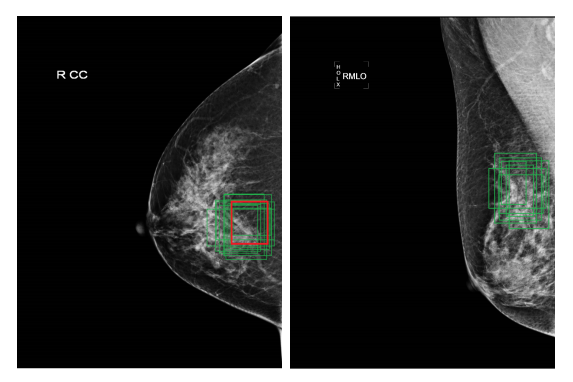
\includegraphics[width=0.6\textwidth]{stage1_anchors}
    \bicaption{经过RPN训练后得到的恶性样本和正常样本预测得到的anchors}{The anchors that were got by RPN after training postive and negative}
    \label{fig:stage1_anchors}
\end{figure}

将负anchors的RPN损失函数定义为最大似然损失:
\begin{equation}
L_{tlloss}=\frac{1}{cls}\sum_{i\in(tops \  p_{i})}L_{cls}(p_{i},p_{i}^{*}=0)
\label{eq1}
\end{equation}

其中,$i$ 是mini-batch中anchors的索引值,$p_{i}$表示的是每个anchor预测为物体的概率值,top likelihood loss只考虑前256个。由于所考虑的是负anchors,所以$p_{i}^{*}$ 的分类标签总是为0。分类损失$L_{cls}$和FasterR-CNN中的RPN网络一样,采用的是交叉熵损失函数。

总而言之,改进后的RPN损失函数定义如下:
\begin{equation}
L_{rpnloss}=L_{ploss} + L_{nloss}= \\
        L_{pclsloss} + {\lambda_1}L_{pregloss} +{\lambda_2}L_{tlloss}
\end{equation}

$L_{ploss}$是针对正样本所考虑的损失函数,和Faster R-CNN中一样,包含分类损失$L_{pclsloss}$和回归损失$L_{pregloss}$。
而对于考虑负样本的$L_{nloss}$,只考虑top likelihood loss $L_{tlloss}$。$\lambda_1,\lambda_2$是调优参数,在本文中设置为1。

\section{Similarity loss}
样本经过RPN训练后和NMS\cite{hosang2017learning}等操作后得到候选框,通过查看RPN得到的候选框(如图\ref{fig:stage1_anchors}所示),可以看出正负anchors所包含的病灶特征高度类似,需要在Fast R-CNN模块尽可能区分开二者。在这部分,本文考虑了人脸识别中常用的孪生网络,也就是学习共享权重网络后的不同类别间的特征向量间的距离。这里引入了similarity loss,并因此改进Faster R-CNN为simFaster R-CNN。
\begin{equation}
L_{simloss}(X_1,X_2)=\frac{1}{K}\sum_{i=1}^{K}\lVert{f(X_1^i)-f(X_2^i)}\rVert
\end{equation}

其中$X_1$和$X_2$ 是从模型Fast R-CNN学习到的特征向量选取而来。负候选框和正候选框共享同一个Fast R-CNN网络权重,$f$是一个距离度量函数,在这里本文主要选择采用cosine函数,降低这个损失函数为了提高识别恶性病灶和疑似恶性病灶的判别能力。但是负候选框是没有病灶信息的。对于所识别出来的疑似恶性病灶的候选框,其分类标签都是为0的,没有回归损失。总的Fast R-CNN损失函数定义如下:

\begin{equation}
L_{fastloss}=L_{clsloss} + {\lambda_3}L_{regloss} +{\lambda_4}L_{simloss}~,
\end{equation}

式子中包括三项:分类损失$L_{clsloss}$,回归损失$L_{regloss}$和similarity loss $L_{simloss}$。$\lambda_3,\lambda_4$ 是调优参数,在本文中设置为1和0.1。


\section{训练过程与细节}
首先对图片进行如第二章的数据预处理操作,之后使用了水平和竖直两种数据扩增方式来降低过拟合。在训练时,本文使用的是基于Resnet101为主干网络的Faster R-CNN,ROI Align的ROI Pooling方式。每次输入的图片是一对数据,分别是从扩增后的恶性数据集和正常数据集分别选择batch\_size 的图片,在每轮取完时,再对相应的数据集进行shuffle,以保证每次取出的数据不一样。本文使用了初始学习率为1e\_4,每经过9k迭代次数下降0.1,总共跑了45k 迭代次数。调优函数使用的是Adam,对于每张图片产生的mini-batch数值设置为128。最终测试时设定的得分置信度为0.5,IoU的置信度选择的是Pascal VOV中的标准值0.5。最终本文使用了Nvidia GTX 1080Ti 两张卡跑了两天左右。

\begin{comment}
其中对于本文数据跑的几个结果的损失下降曲线如下\ref{fig:1_stage_loss}。

\begin{figure}[!htbp]
    \centering
    \begin{subfigure}[a]{1.0\textwidth}
      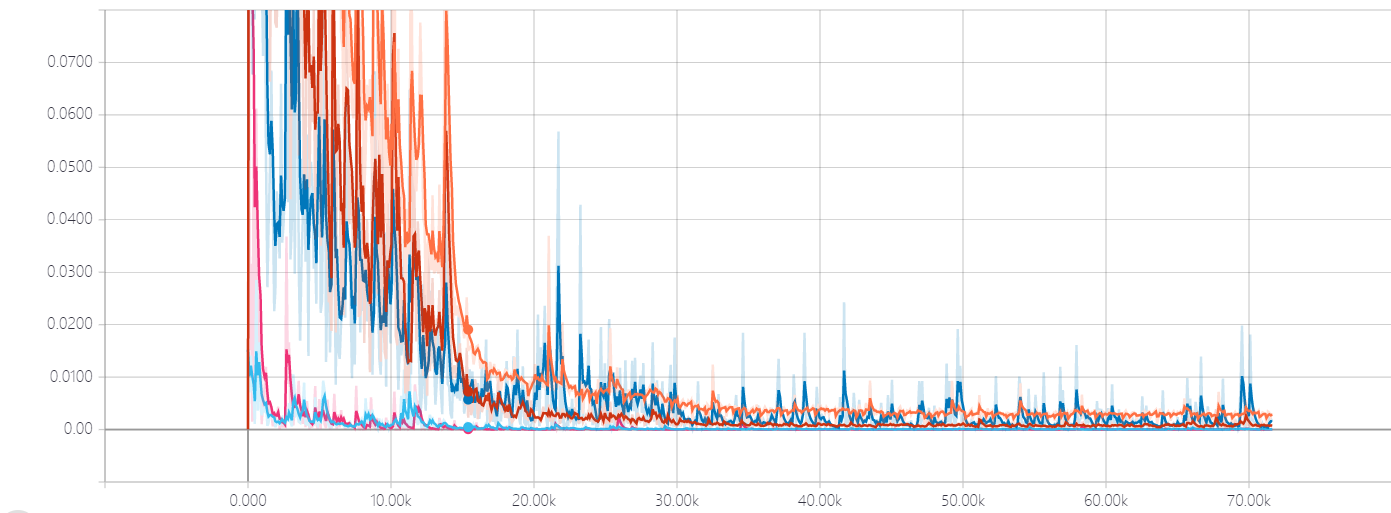
\includegraphics[width=\textwidth]{stage1_fa}
      \caption{}
      \label{fig:stage1_fa}
    \end{subfigure}%
    
    ~% add desired spacing
    \begin{subfigure}[b]{1.0\textwidth}
      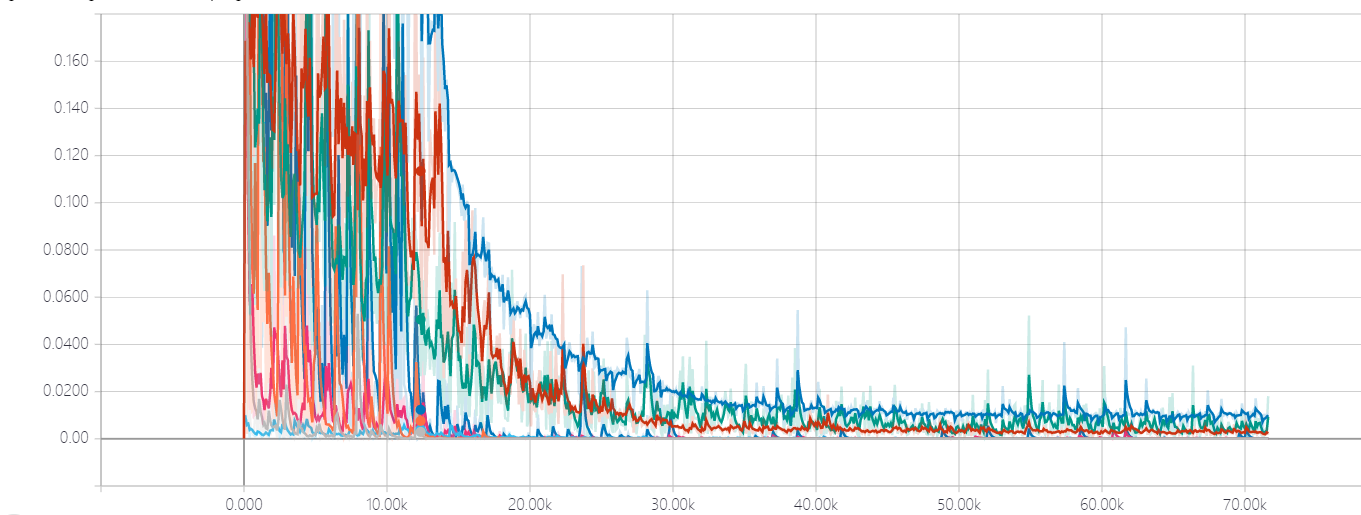
\includegraphics[width=\textwidth]{stage1_fa_tl}
      \caption{}
      \label{fig:stage1_fa_tl}
    \end{subfigure}
    
    \begin{subfigure}[c]{1.0\textwidth}
      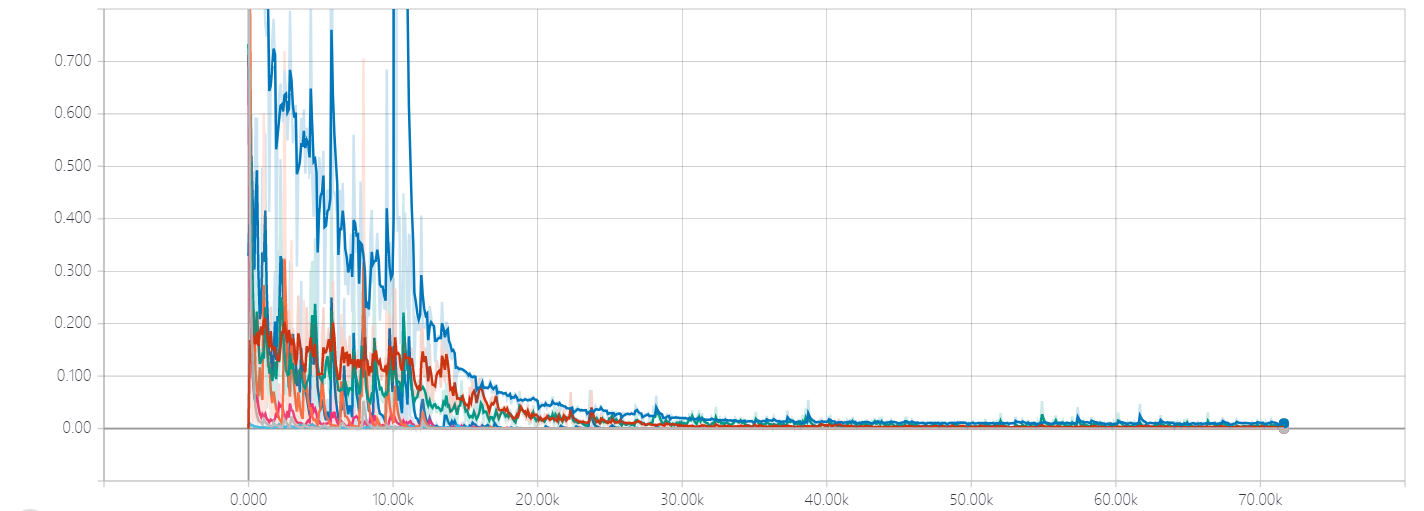
\includegraphics[width=\textwidth]{stage1_fa_tl_sim}
      \caption{}
      \label{fig:stage1_fa_tl_sim}
    \end{subfigure}

    \bicaption{一阶段不同模型的损失下降曲线图(a) Faster R-CNN 模型loss下降图(b) Faster R-CNN + tlloss模型loss下降图 (c)simFaster R-CNN模型loss下降图}
    {The loss curve for different models for 1-stage model (a) loss curve for Faster R-CNN (b) loss curve for Faster R-CNN + tlloss (c)loss curve for Faster R-CNN + tlloss + simloss}
    \label{fig:1_stage_loss}
\end{figure}
\end{comment}

\section{结果讨论与分析}
\subsection{基于病例}
对运行各个结果显示如表\ref{tab:1_stage_pred_result_based_on_patient}所示。

\begin{table}[!htbp]
    \bicaption{simFaster R-CNN基于病例预测结果}{
The prediction results of simFaster R-CNN based on patient}
    \label{tab:1_stage_pred_result_based_on_patient}
    \centering
    \footnotesize% fontsize
    \setlength{\tabcolsep}{4pt}% column separation
    \renewcommand{\arraystretch}{1.2}%row space 
    \begin{tabular}{ccccc}
        \hline
        &AUC& ACC &SEN &SPE\\
        \hline
        Faster R-CNN& 0.8467 &0.7622 &0.9667 &0.6145 \\
        Faster R-CNN+tlloss& 0.8696 &0.8531 &0.8333 &0.8675 \\
        simFaster R-CNN& 0.9110 &0.8881 &0.9167 &0.8675 \\
        \hline
    \end{tabular}
\end{table}

从上到下的模型依次是使用原始的Faster R-CNN模型直接对正负样本进行训练,对负样本添加top likelihood loss的Faster R-CNN模型(Faster R-CNN+tlloss),对负样本同时添加top likelihood loss和similarity loss的simFaster R-CNN模型(Faster R-CNN+tlloss+similoss)。

模型最终预测得到的ROC曲线如图\ref{fig:stage1_auc}。
		\begin{figure}[!htbp]
    \centering
    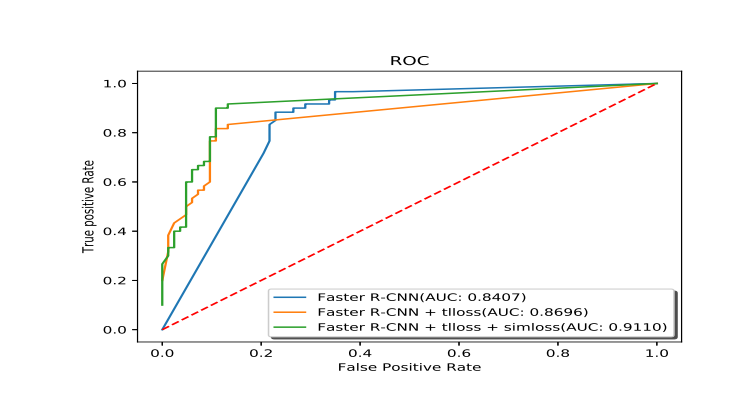
\includegraphics[width=1.0\textwidth]{stage1_auc}
    \bicaption{simFaster R-CNN ROC曲线}{The ROC curve of simFaster R-CNN}
    \label{fig:stage1_auc}
	\end{figure}
从结果上可以看出,原始的Faster R-CNN模型由于缺乏对负样本的有效学习,使得在最终评判标准上存在敏感度上高,但特异度上很低的情况。
在上述原始模型上添加了top likelihood loss之后,模型虽然对于正样本的敏感度下降了,但是对于负样本的特异度提升,这表明该loss能够有效帮助模型更好地学习负样本的信息。
最后,添加了专门学习正样本和负样本差异性的similarity loss后,模型在保持特异度不变的情况下,有效提高了敏感度。
本文设计的top likelihood loss和similarity loss在各个指标都取得了远远超过原始的FasterR-CNN的结果,最终AUC可以达到0.91,甚至超过了临床诊断上医生的识别率0.72。
这结果充分表明了simFaster R-CNN通过添加top likelihood loss来降低RPN中被判错的负anchors,以及通过similarity loss来学习不同类别的微小差异的有效性,进而能够在满足精度的情况下,提升了模型的训练速度。
	
\subsection{基于图片}
\begin{table}[!htbp]
    \bicaption{simFaster R-CNN基于图片预测结果}{
The prediction results of simFaster R-CNN based on image}
    \label{tab:1_stage_pred_result_based_on_image}
    \centering
    \footnotesize% fontsize
    \setlength{\tabcolsep}{4pt}% column separation
    \renewcommand{\arraystretch}{1.2}%row space 
    \begin{tabular}{cc}
        \hline
        &mAP\\
        \hline
        Faster R-CNN& 0.4055\\
        Faster R-CNN+tlloss& 0.4219\\
        simFaster R-CNN& 0.5353\\
        \hline
    \end{tabular}
\end{table}
本文还对比了传统的mAP指标,该指标综合考虑了单张图片中各个预测框的分类和检测性能。从表\ref{tab:1_stage_pred_result_based_on_image}中可以看出,该结果也是随着模型的不断完善和优化而不断提升的,并最终在本文提出的simFaster R-CNN达到最优的结果。

综合对比weakFaster R-CNN的结果(如表\ref{tab:2_stage_2_pred_result}),可知simFaster R-CNN在AUC,SEN,mAP等指标超过了weakFaster R-CNN,体现出其优越的性能。weakFaster R-CNN由于第二阶段能够使用初步筛选的疑似恶性乳腺钼靶数据作为训练数据,所以其在良性样本的区分度能力更强,也就是SPE指标上会比simFaster R-CNN数值高一点。但整体而言,simFaster R-CNN耗时少,不占用大量空间,取得了不输于weakFaster R-CNN的性能。
\begin{table}[!htbp]
    \bicaption{weakFaster R-CNN预测结果}{
The prediction results of weakFaster R-CNN}
    \label{tab:2_stage_2_pred_result}
    \centering
    \footnotesize% fontsize
    \setlength{\tabcolsep}{4pt}% column separation
    \renewcommand{\arraystretch}{1.2}%row space 
    \begin{tabular}{cccccc}
        \hline
        &AUC& ACC &SEN &SPE &mAP\\
        \hline
        weakFaster R-CNN& 0.8467 &0.9123 &0.8846 &0.9123 &0.4055\\
        simFaster R-CNN& 0.9110 &0.8881 &0.9167 &0.8675 &0.5353\\
        \hline
    \end{tabular}
\end{table}

\subsection{可视化预测结果}
模型对于正样本预测结果如图\ref{fig:stage1_vis},从左到右分别是Faster R-CNN,Faster R-CNN+tlloss, simFaster R-CNN对正样本的预测结果,其中黄框为真实框,粉红框为预测框。可以看出,随着模型的不断优化,模型对于postive的分类以及回归的精度都得到有效的提升。添加的top likelihood loss可以有效降低负anchors的召回率,降低anchors的假阳性率,从而提高模型的性能。添加similiarity loss由于考虑了正负样本的微弱差异,在定位精度上会比只加top likelihood loss更高。
		\begin{figure}[!htbp]
    \centering
    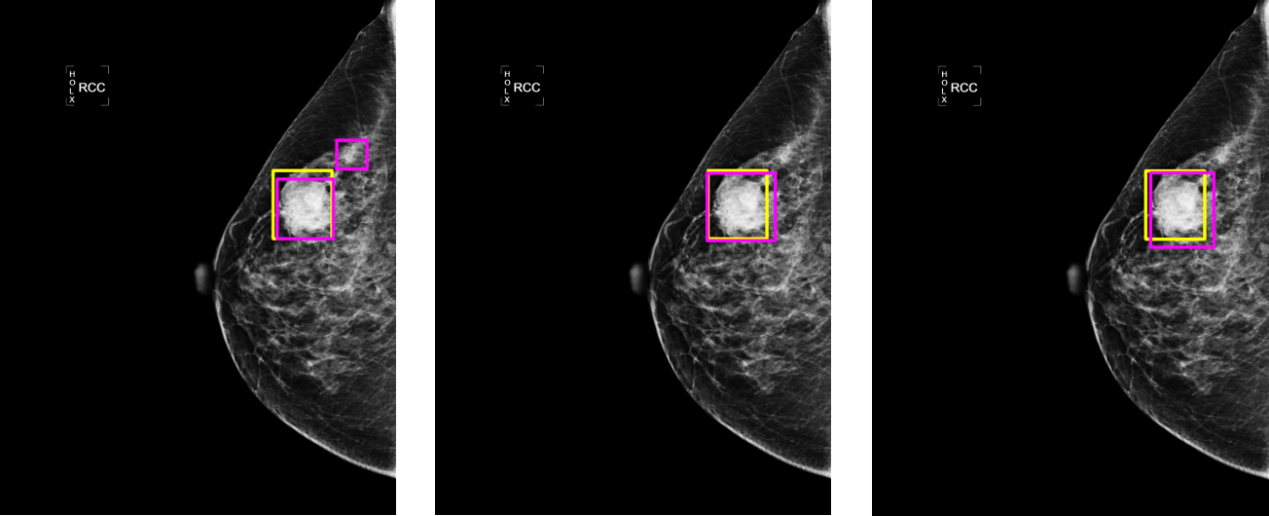
\includegraphics[width=0.70\textwidth]{stage1_vis}
    \bicaption{simFaster R-CNN在天肿数据集上的对正样本预测结果可视化}{The detection results of positive in vision using simFaster R-CNN at the tianzhong datasets}
    \label{fig:stage1_vis}
	\end{figure}
		
对于负样本预测结果如图\ref{fig:stage1_vis_neg},从左到右分别是Faster R-CNN,Faster R-CNN+tlloss, simFaster R-CNN对负样本的预测结果,其中粉红框为预测框。从对于负样本上的结果上看,可以清晰地看出模型对于负样本的识别能力随着loss的添加而不断地提升。原始的Faster R-CNN存在很明显的高假阳性率,而且其得到的高度疑似恶性病灶的预测框定位并不够精准。添加了top likelihood loss会在一定程度上提高模型的定位精度。当使用了similarity loss后的simFaster R-CNN则同时在分类和定位上远远超过最原始的Faster R-CNN,从而极大地降低了模型的假阳性率。
	
	\begin{figure}[!htbp]
    \centering
    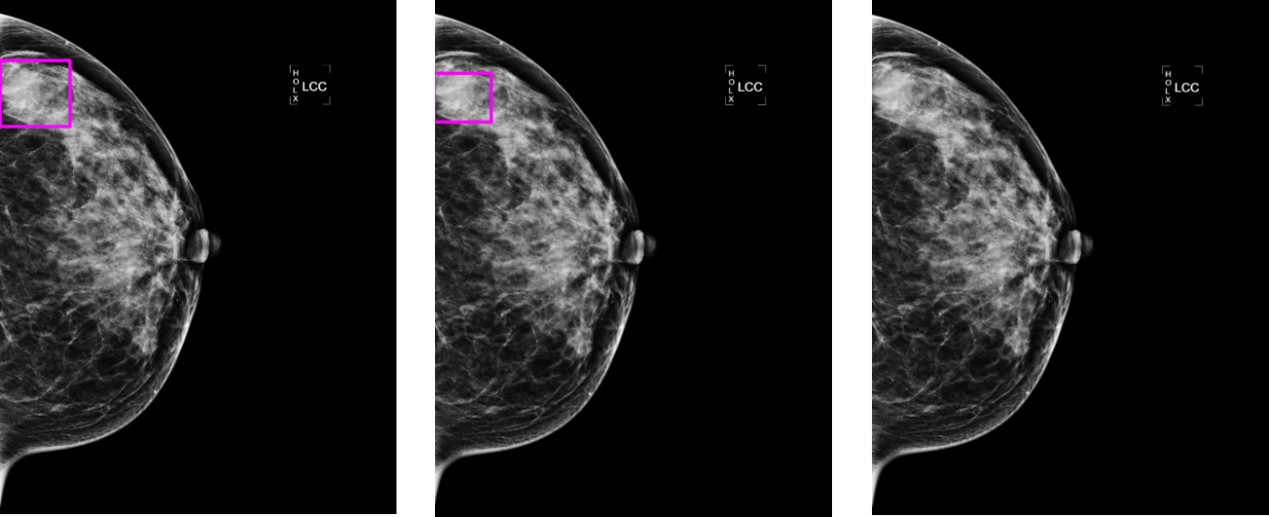
\includegraphics[width=0.7\textwidth]{stage1_vis_neg}
    \bicaption{simFaster R-CNN在天肿数据集上的对负样本预测结果可视化}{The detection results of negative in vision using simFaster R-CNN at the tianzhong datasets}
    \label{fig:stage1_vis_neg}
	\end{figure}
	
	总而言之,随着loss的不断添加,模型对于恶性的分类及定位,对于正常样本的分类都有了更加精准的提升。这也很好地佐证了上述模型的指标大幅提升。
\section{其他工作}
本文还进行了诸多的尝试,比如修改模型的主干网络,用其他的similarity loss,修改调优函数,主干网络上添加模块等操作,其他公开数据集上的比较。
\subsection{更换主干网络}
本文还对比分析了最后一届ILSVR的冠军模型Senet\cite{64hu2018squeeze},top5的错误率达到了2.251\%,比2016年的第一名还要低25\%,其主要考虑了各个特征层之间的关系,通过学习各个特征层不同的权重并应用注意里机制,使得关键特征层可以凸显发挥更大的作用。其重要的SE Block如图\ref{fig:stage1_senet}所示。
			\begin{figure}[!htbp]
    \centering
    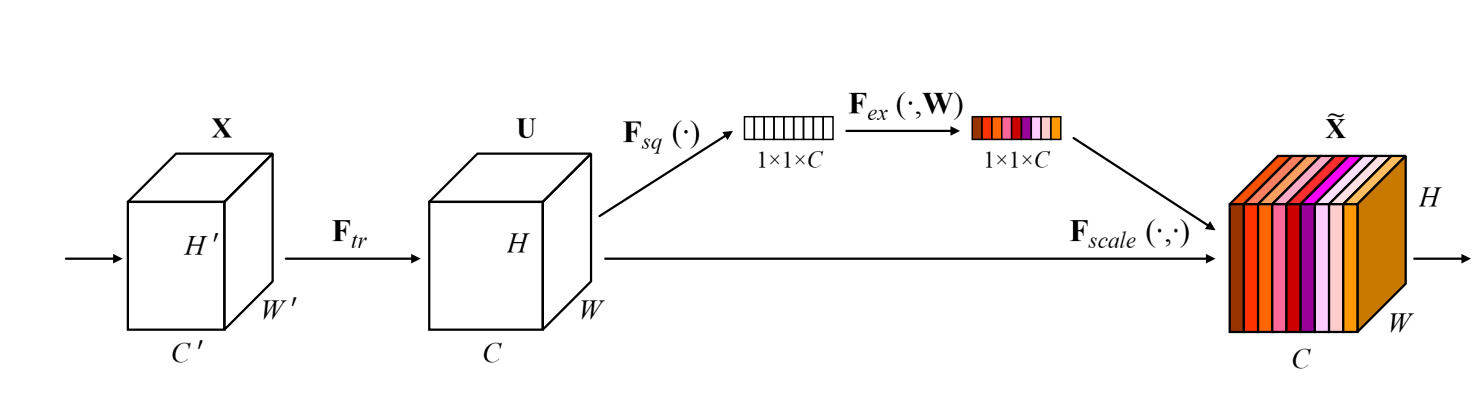
\includegraphics[width=1.0\textwidth]{stage1_senet}
    \bicaption{SE Block\cite{64hu2018squeeze}}{SE Block\cite{64hu2018squeeze}}
    \label{fig:stage1_senet}
	\end{figure}
	
同上,本文取Seresnet101作为模型的主干网络,从结果(如表\ref{tab:1_stage_senet_pred_result})可以看出,Seresnet101作为主干网络对于最终结果,并没有达到或超过Resnet101的效果。分析原因可能是,传统的自然图像是三通道的,其各个通道之间存在关联信息,使得SE Block可以在其中发挥作用,而对于乳腺钼靶数据,其原始图片为单通道灰度图信息,单纯地通过通道叠加变成RGB三通道,Seresnet101并没有学习通道之间的关系,进而不能够对不同通道施加不同权重。Seresnet101引入额外计算,使得模型在时间复杂度上会比Resnet101更高。
\begin{table}[!htbp]
    \bicaption{simFaster R-CNN使用Seresnet101模型预测结果}{
The prediction results of simFaster R-CNN using Seresnet101 as backbone}
    \label{tab:1_stage_senet_pred_result}
    \centering
    \footnotesize% fontsize
    \setlength{\tabcolsep}{4pt}% column separation
    \renewcommand{\arraystretch}{1.2}%row space 
    \begin{tabular}{ccccc}
        \hline
        AUC& ACC &SEN &SPE &mAP \\
        \hline
        0.8505 &0.7972 &0.8785  &0.7762 &0.3865 \\
        \hline
    \end{tabular}
\end{table}

\subsection{更换similarity loss}
孪生网络训练中所采用的loss是contrastive loss。这种损失函数可以有效的处理孪生神经网络中的数据对的关系,传统的Siamese network使用contrastive loss,其函数如下:
\begin{equation}
	\operatorname{con}_{-} \operatorname{loss}=(1-Y) \frac{1}{2}\left(D_{w}\right)^{2}+(Y) \frac{1}{2}\left\{\max \left(0, m-D_{w}\right)\right\}^{2}
\end{equation}

\begin{itemize}
	\item $D_{w}$被定义为姐妹孪生网络的输出之间的欧氏距离。 $D_{w}$欧式距离公式如下:
		\begin{equation}
			\cos _{-} \operatorname{loss}=\sqrt{\left\{G_{w}\left(X_{1}\right)-G_{w}\left(X_{2}\right)\right\}^{2}}
		\end{equation}
	\item $G_{w}$是其中一个姐妹网络的输出。$X_{1}$和$X_{2}$是输入数据对。
	\item $Y$值为1或0。如果模型预测输入是相似的,那么$Y$的值为0,否则$Y$为1。
	\item $max$是表示0和$m-D_{w}$之间较大值的函数。
	\item $m$是大于0的边际价值(margin value)。有一个边际价值表示超出该边际价值的不同对不会造成损失。
	
\end{itemize}

\begin{comment}
其表达式如下:
\begin{equation}
	L\left(W,\left(Y, X_{1}, X_{2}\right)\right)=\frac{1}{2 N} \sum_{n=1}^{N} Y D_{W}^{2}+(1-Y) \max (m-D w, 0)^{2}
\end{equation}

其中$D \mathrm{w}=\left\|X_{1}-X_{2}\right\|_{2}=\left(\sum_{i}^{N}\left(X_{1}^{i}-X_{2}^{i}\right)^{2}\right)^{\frac{1}{2}}$表示样本特征$X_1$和$X_2$的欧式距离,$Y$为两个样本是否匹配的标签,$Y=1$代表两个代表两个样本相似或者匹配, $Y=0$代表不匹配, $m$为设定的阈值。
\end{comment}
相比于cosine loss, 该loss考虑了多种数据对情况,包括同正,同负,一正一负等。从结果(如表\ref{tab:1_stage_con_pred_result})可以看出
该loss对比于cosine loss,除了SPE指标外均取得了超过cosine loss的结果。对于本文而言,最终所要考虑的仅是一正一负这种情况,这使得该loss对于不同类别之间的区别学习比较充分,而对于同类别,尤其是同负类的相似度学习并不充分,所以更多地推远了恶性样本和正常样本(一正一负)的距离,而并没有有效的拉近恶性样本(同正)或正常样本(同负)之间的距离,在结果上表现为AUC和mAP会比cosine来的大,但对于SEN和SPE并没有太大的提升。

\begin{table}[!htbp]
    \bicaption{simFaster R-CNN使用contrastive loss预测结果}{
 The prediction results of simFaster R-CNN using  contrastive loss as similarity loss}
    \label{tab:1_stage_con_pred_result}
    \centering
    \footnotesize% fontsize
    \setlength{\tabcolsep}{4pt}% column separation
    \renewcommand{\arraystretch}{1.2}%row space 
    \begin{tabular}{ccccc}
        \hline
        AUC& ACC &SEN &SPE &mAP \\
        \hline
        0.9262 &0.8042 &0.9500  &0.6988 &0.5525 \\
        \hline
    \end{tabular}
\end{table}


\subsection{更换权重因子}
$\lambda_{1}$, $\lambda_{2}$, $\lambda_{3}$, $\lambda_{4}$为调节各个loss权重的因子,通过调节不同情况下各个值,可以达到突出或者降低某个loss影响的作用。在本文中,默认使用的其值分别是$\lambda_{1}$=1,$\lambda_{2}$=1,$\lambda_{3}$=1,$\lambda_{4}$=1。为了更好地挖掘这些因子的作用,本文还进行了以下的对比实验。如表\ref{tab:1_stage_lambda_pred_result}所示。
\begin{table}[!htbp]
    \bicaption{simFaster R-CNN使用不同权重因子预测结果}{
 The prediction results of simFaster R-CNN using different lambda}
    \label{tab:1_stage_lambda_pred_result}
    \centering
    \footnotesize% fontsize
    \setlength{\tabcolsep}{4pt}% column separation
    \renewcommand{\arraystretch}{1.2}%row space 
    \begin{tabular}{cccccc}
        \hline
        &AUC& ACC &SEN &SPE &mAP \\
        \hline
        $\lambda_{1}$=1, $\lambda_{2}$=0.9, $\lambda_{3}$=1, $\lambda_{4}$=0.1&0.9036 &0.8811 &0.8833  &0.8795 &0.5266 \\
        $\lambda_{1}$=1, $\lambda_{2}$=0.1, $\lambda_{3}$=1, $\lambda_{4}$=0.9&0.8641 &0.8531 &0.8333  &0.8675 &0.5094 \\
        \hline
    \end{tabular}
\end{table}

可以看出,不同的$\lambda_{1}$, $\lambda_{2}$, $\lambda_{3}$, $\lambda_{4}$值对于结果影响较大,在本文数据中最好的参数依然是$\lambda_{1}$=1,$\lambda_{2}$=1,$\lambda_{3}$=1,$\lambda_{4}$=1。而对于后期的DDSM数据,最好的权重因子参数分别是$\lambda_{1}$=1,$\lambda_{2}$=0.9,$\lambda_{3}$=1,$\lambda_{4}$=0.1。不同的参数会对模型最终训练效果产生影响,这需要在实验中进行具体的尝试。

\subsection{添加模块}
对数据进行纵横比查看,如图\ref{fig:stage1_aspect}分析,发现其纵横比落在1:2,1:1和2:1三个区间内,且由于乳腺钼靶本身图片像素大,造成的缩放比影响较大。打算使用Deformable Convolutional Network(DCN)\cite{66dai2017deformable},通过卷积核的学习来对这种影响进行修正。DCN通过考虑对卷积核中每个采样点的位置添加了一个偏移的变量,通过这些变量,卷积核可以在当前位置附近随意的采样,而不再局限于之前的规则格点。
\begin{figure}[!htbp]
    \centering
    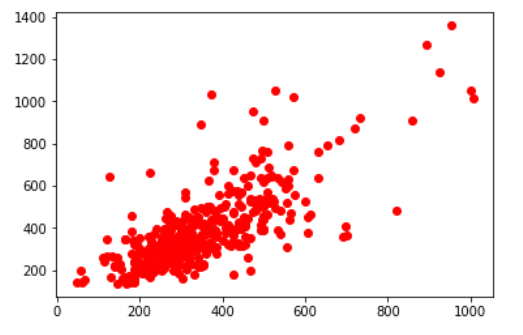
\includegraphics[width=0.7\textwidth]{stage1_aspect}
    \bicaption{乳腺钼靶纵横比}{Aspect ratio of mammography}
    \label{fig:stage1_aspect}
\end{figure}

通过使用DCN模块,从最终结果(如表\ref{tab:1_stage_dcn_pred_result})可以看出,DCN在结果上并没有太大优势。DCN的提出是由于传统自然图像上存在超过正常三种纵横比之外的其他纵横比,而对于乳腺钼靶数据而言,纵横比的差异不够突出,DCN在这方面并没有发挥出他的作用。
\begin{table}[!htbp]
    \bicaption{simFaster R-CNN添加DCN模块预测结果}{
 The prediction results of simFaster R-CNN adding DCN}
    \label{tab:1_stage_dcn_pred_result}
    \centering
    \footnotesize% fontsize
    \setlength{\tabcolsep}{4pt}% column separation
    \renewcommand{\arraystretch}{1.2}%row space 
    \begin{tabular}{ccccc}
        \hline
        AUC& ACC &SEN &SPE &mAP \\
        \hline
        0.8149 &0.6923 &0.8833  &0.5542 &0.4893 \\
        \hline
    \end{tabular}
\end{table}

\subsection{更换数据集}
针对这种方法,我还扩展对比了在DDSM上的表现。DDSM数据库是由南佛罗里达大学创建并一直如此广泛用于乳房研究目的,它包含2620案件分为43卷,每张乳腺钼靶照片包含与之相关的可疑病变的信息。对于恶性图片如图\ref{fig:stage1_ddsm}所示。
\begin{figure}[!htbp]
    \centering
    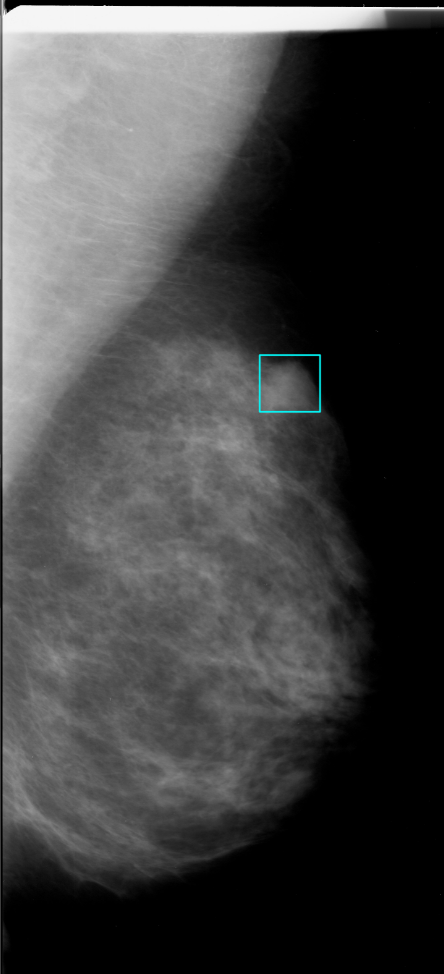
\includegraphics[height=0.40\textwidth]{stage1_ddsm}
    \bicaption{DDSM乳腺钼靶图}{DDSM Mammography}
    \label{fig:stage1_ddsm}
\end{figure}

相对于本文的东方女性致密性乳腺,DDSM的乳腺钼靶更多是西方女性的少量腺体型乳腺。使用不同数据集是为了判断模型simFaster R-CNN是否具有迁移不同知识的能力。

按照AL-MASNI M A等\cite{al2017detection}中对DDSM进行去除存在问题的图片和采集数据,本文最后取出DDSM中的包含肿块的部分数据集,训练集中包括600张图片,其中304张是带有病灶坐标标记信息的恶性样本,296张不带有标记信息,也就是正常样本;测试集中包括100张图片,其中45张带有标注信息的恶性样本,55张为不带有标记信息的正常样本,数据划分如表\ref{tab:data_set_split for ddsm}所示。
\begin{table}[!htbp]
    \bicaption{DDSM数据集划分}{Data set partition of DDSM}
    \label{tab:data_set_split for ddsm}
    \centering
    \footnotesize% fontsize
    \setlength{\tabcolsep}{4pt}% column separation
    \renewcommand{\arraystretch}{1.2}%row space 
    \begin{tabular}{ccc}
        \hline
        数据集& 带病灶恶性图片数& 正常样本数\\
        \hline
        训练集& 304 &296\\
		\hline
		测试集& 45 &55\\
        \hline
    \end{tabular}
\end{table}

按照和本文数据一样的数据方式,最终对结果进行预测如表\ref{tab:1_stage_ddsm_pred_result}所示。
\begin{table}[!htbp]
    \bicaption{simFaster R-CNN使用DDSM数据集基于图片预测结果}{
The prediction results of simFaster R-CNN using DDSM as dataset based on image}
    \label{tab:1_stage_ddsm_pred_result}
    \centering
    \footnotesize% fontsize
    \setlength{\tabcolsep}{4pt}% column separation
    \renewcommand{\arraystretch}{1.2}%row space 
    \begin{tabular}{ccccc}
        \hline
        &AUC& ACC &SEN &SPE \\
        \hline
        Faster R-CNN(no annotation on benign) &0.8945 &0.8100 &0.8667 &0.7636\\
       	simFaster R-CNN &0.9446 &0.9300 &0.9111  &0.9455  \\
       	Faster R-CNN(with annotated benign) &0.9269 &0.9100 &0.8667  &0.9455  \\
       	AL-MASNI M A等\cite{al2017detection} &0.8774 &0.8552 &0.9320  &0.7800  \\
        \hline
    \end{tabular}
\end{table}

考虑到与AL-MASNI M A等\cite{al2017detection}的预测结果进行对比,所以这里计算的所有指标都是基于图片上进行考量。可以看出一阶段模型simFaster R-CNN在各个指标上远远超过原始的Faster R-CNN(no annotation on benign)。在AUC、ACC、SPE均超过AL-MASNI M A等\cite{al2017detection}的,SEN较低原因在于本模型需要考虑到负样本情况,而AL-MASNI M A等\cite{al2017detection}是在基于标注信息训练的最终结果。同时,本文还在弱监督上训练的模型与带有全部标注信息的Faster R-CNN(with annotated benign)进行对比,发现结果并不差,这很好的证明了simFaster R-CNN想法的有效性。

对DDSM的正样本(如图\ref{fig:stage1_ddsm_vis})及负样本(如图\ref{fig:stage1_ddsm_vis_neg})预测结果进行可视化(取置信度为0.5,从左到右分别是Faster R-CNN,Faster R-CNN+tlloss, simFaster R-CNN)对DDSM正样本的预测结果,其中黄框为真实框,粉红框为预测框。从结果中可以看出,随着loss的不断增加,模型对于病灶的预测假阳性率不断下降,而且定位精度不断提升,从而也有效证明了simFaster R-CNN具备数据迁移学习的强大能力。
		\begin{figure}[!htbp]
    \centering
    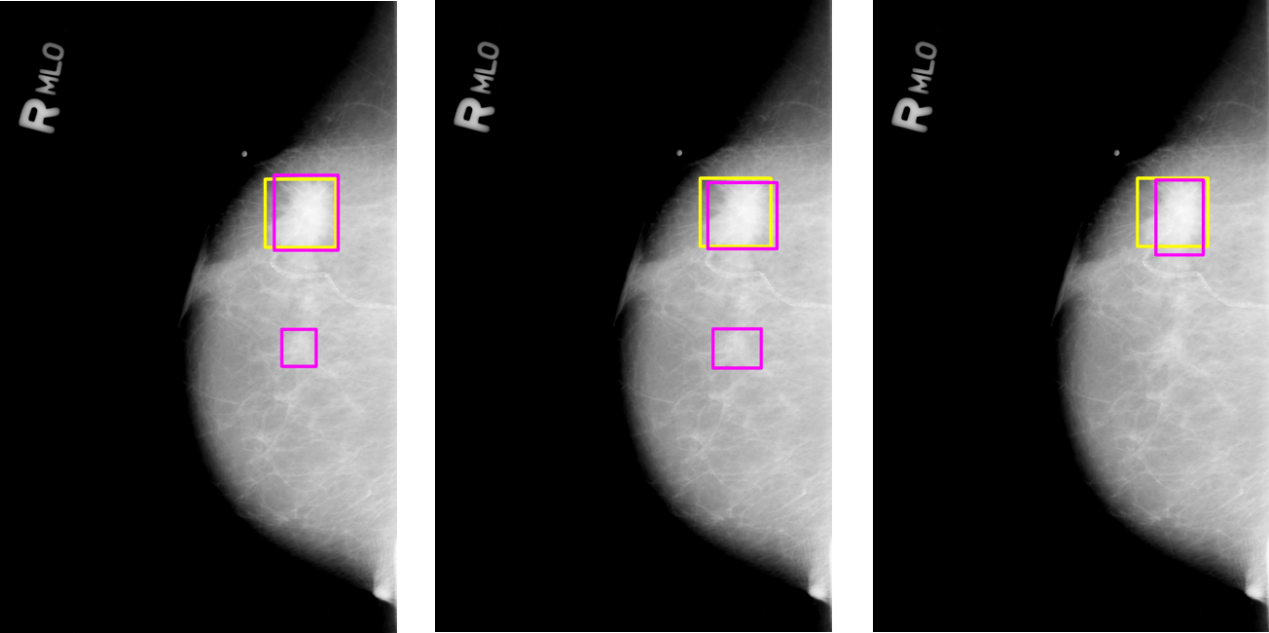
\includegraphics[width=0.7\textwidth]{stage_1_mal}
    \bicaption{simFaster R-CNN在DDSM数据集上的对正样本预测结果可视化}{The detection results of positive in vision using simFaster R-CNN based on the DDSM datasets}
    \label{fig:stage1_ddsm_vis}
	\end{figure}
	
	\begin{figure}[!htbp]
    \centering
    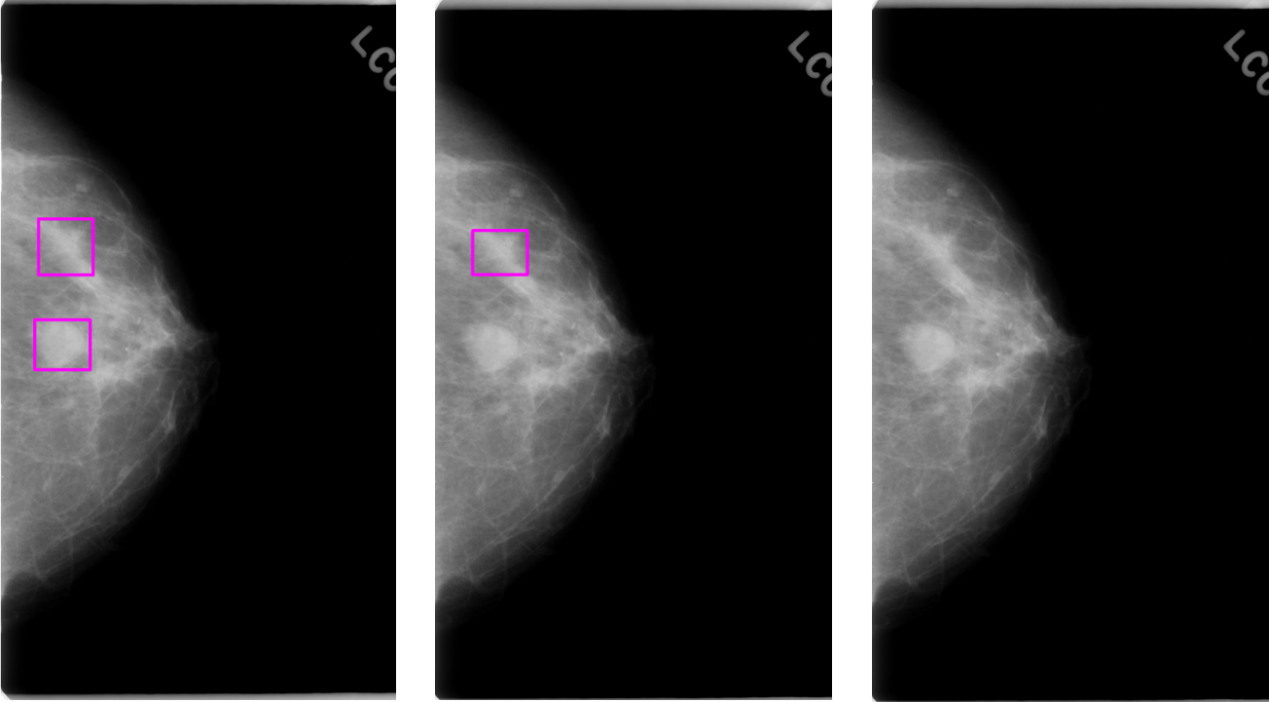
\includegraphics[width=0.7\textwidth]{stage1_ddsm_ben}
    \bicaption{simFaster R-CNN在DDSM数据集上的对负样本预测结果可视化}{The detection results of negative in vision using simFaster R-CNN based on the DDSM datasets}
    \label{fig:stage1_ddsm_vis_neg}
	\end{figure}

\section{本章小结}
本章在对两阶段的劣势分析的基础上,全新设计了一阶段模型simFaster R-CNN,其中正样本和负样本共享主干网络,RPN网络及Fast R-CNN网络。在RPN阶段,对大量拥有高度疑似恶性信息的负anchors进行损失考虑,降低其对真正的正anchors的影响;在Fast R-CNN阶段,本章引入similarity loss,着重学习区分恶性样本和正常样本之间的差异,从而提升模型的性能。本章还对simFaster R-CNN进行了各种尝试的改良工作,并在公开的大型数据集DDSM上与其他人的工作进行了对比分析。